
%%% Local Variables:
%%% mode: latex
%%% TeX-master: t
%%% End:

\chapter{基于自适应正例去噪的推荐算法研究}
\label{cha:2}
对于个性化推荐应用而言,最广泛使用的隐式反馈是一种不完全数据(Incomplete Data),只能观察到交互的有无,而无法观察到该交互所对应偏好的大小。隐式反馈数据中通常包含一些不可信交互(误报),即伪正例,例如代购、误触等交互数据。由这些伪正例构建的成对比较,是不可信的成对比较,也称为含噪声成对比较,导致成对学习模型的不准确优化。本章提出一种自适应去噪的成对排序推荐算法(Bayesian Personalized Ranking with Autonomous Credence, BPRAC),用于从含噪成对比较的数据中学习个性化排序。由于交互对应的偏好值不可观测,本章引入一个隐变量作为衡量交互置信度的新指标,这个隐变量与用户物品表示一起作为模型参数进行端到端地学习。所提出的BPRAC算法采用期望最大化框架:在期望步骤中使用贝叶斯推断来估计交互的置信度指标;在最大化步骤中固定置信度指标,更新参数学习用户和物品的表示。在真实世界的数据集上进行的实验验证了所提出的算法的有效性。

\section{引言}
\begin{figure}[!htbp]
	\centering
	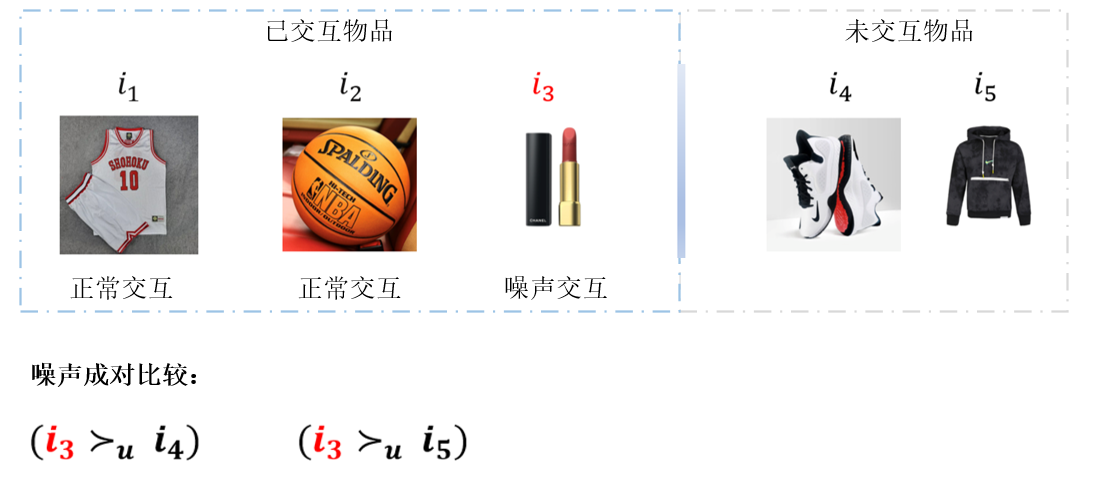
\includegraphics[width=0.6\textwidth]{2-IllustrativeExample.png}
	\caption{含噪成对比较示意图}
	\label{Fig2-1}
\end{figure}

首先用一个直观的例子阐释推荐系统中的正例噪声问题。如图~\ref{Fig2-1}所示,一个运动爱好者在节日期间购买了一个口红$i_3$作为礼物,这是一个不体现该用户偏好的偶然交互行为。但是隐式反馈数据并不包含交互所对应的偏好值,推荐模型无法识别这种不体现用户偏好的异常交互模式。成对比较是由已经交互的正例和未交互的负例构成,由于$i_3$是伪正例,任何包含$i_3$的成对比较,都是噪声成对比较。由此构成的优化目标,导致模型误认为该运动爱好者更偏好口红而非其他运动物品。协同过滤机制又会导致与口红类似的女性用品被推荐给该用户,造成过高的伪正例率。

一般而言,存在两种类型的噪声:一种是特征依赖的噪声\cite{Menon:2018:ML},例如标注者可能倾向于混淆狼和狗,但不会混淆老虎和狗,因此狼容易被错误标注而老虎不会;另外一种是独立于特征的噪声\cite{patrini:2017:CVPR},如高斯白噪声。推荐系统的误报兼具二者特征。例如误触,与物品的特征无关,每个交互的噪声率是随机分布的;而代购,则与物品的特征有关,具有礼物性质的物品更容易产生较高的噪声率。噪声来自多个方面,包括数据收集过程中的错误、不准确的标注、不完整的数据、异常值等。隐式反馈数据是典型的不完全数据,只能观测到用户的交互记录,但是无法观测到交互所对应偏好的高低。隐式反馈数据中存在一些不体现用户偏好的误触、代购等异常交互模式,和其它正常交互被无差别记录,导致了伪正例问题。噪声对机器学习模型的性能和泛化能力的负面影响体现在多个方面。首先,噪声可能导致模型对数据的过拟合。模型可能会将噪声视为真实模式,从而导致错误的学习和预测。其次,噪声可能降低模型的准确性和稳定性。如果训练数据包含大量噪声,模型可能无法准确地捕捉数据的真实分布和模式,从而导致预测结果的不可靠性。

先前的研究主要是从数据、目标函数和优化策略的角度出发解决正例噪声问题,并提出了相应的解决方法和技术。具体而言,从数据的角度,重点是通过图数据增强\cite{pmlr-v119-zheng20d,10.1145/3437963.3441734,10.1145/3437963.3441720,page1998pagerank},以获取体现原始用户物品二分图结构信息的增强图,从而有助于消除噪声正例的影响。从目标函数的角度出发,主要思路是经验风险重写(Empirical Risk Rewriting)。例如文献~\cite{liu2015classification}和文献\cite{xia:2019:NIPS}通过重加权样本,重写能够容忍噪声的损失函数,它比标准损失函数更具鲁棒性。最后,从优化策略的角度出发,重点是探索优化的动态过程,以解决标签噪声学习问题。核心在于,神经网络倾向于先拟合干净数据,然后拟合噪声数据\cite{zhang2021understanding}。基于这一发现,例如早停法~\cite{li2020gradient}作为一种简单而有效的方法,用于避免在噪声数据上过拟合;而Co-teaching方法~\cite{Han:2018:NIPS}通过小损失技巧相互筛选干净样本,鲁棒地同时训练两个网络。

在成对学习的问题设置下,正例噪声问题更具挑战性。从优化策略出发的“神经网络倾向于先拟合干净数据,然后拟合噪声数据”的经验性观察主要是基于单个样本构建的损失,是否在成对样本构建的损失上依旧起作用是存疑的,因为在推荐中往往是难以拟合的困难样本对性能的提升贡献越大\cite{Steffen:2014:WSDM}。从数据角度出发的图数据增强可能会损失图中重要的结构信息,因为随机丢弃的点或者边可能会体现图的重要结构信息,从而引入新的噪声。从目标函数角度出发的经验函数重写,主要是基于以均方误差等为代表点式损失(pointwise)损失,这类损失在单个样本和标签上构建,难以向对比损失推广。

回溯伪正例的本质,是隐式反馈数据的特性造成的
:它是一种不完全数据,无法观测到交互所对应的偏好值,才产生了噪声成对比较。如果能观测到每个交互偏好强度的高低,那么根据偏好值大小值构造的成对比较就是可靠的。从统计视角,期望-最大化(Expectation-Maximazation)最大化框架是一个从不完全数据中进行极大似然或者最大后验估计非常有效的方法,可以估计无法观测到的隐变量和模型参数。因此,本章引入一个隐变量,含义为每个交互的偏好值,同时也对应了每个成对比较置信度的高低,交互的偏好值越大则成对比较的置信度越高,并端到端地学习模型参数和置信度指标:在期望步骤中使用贝叶斯推断来估计置信度指标;在最大化步骤中固定置信度指标,更新模型参数学习用户和物品的表示,以减少噪声成对比较对学习算法的影响,学习更加准确的用户和物品表示。

本章对推荐系统的正例去噪研究做出了如下贡献:(1)将从噪声成对比较中学习排序形式化为一个含有隐变量的最大后验估计问题;(2)贡献了基于次序统计量的排序分析的隐变量估计方法。

\section{自适应正例去噪算法设计}
\subsection{问题设置}
设$\mathbf{X}=[x_{ui}] \in \mathbb{R}^{M\times N}$表示包含$M$个用户和$N$个物品的交互矩阵,其中$x_{ui}\in \{1,0\}$。令$\mathcal{U}$和$\mathcal{I}$分别表示用户集合和物品集合。对于用户$u \in \mathcal{U}$,令$\mathcal{I}_u^+ \subseteq \mathcal{I}$表示他交互过的物品集合,$\mathcal{I}_u^- = \mathcal{I}\backslash \mathcal{I}_u^+$表示他未交互过的物品集合。通过选择一个属于$\mathcal{I}_u^+$的物品$i$和一个属于$\mathcal{I}_u^-$的物品$j$,可以构建成对比较的实例。训练数据集可以通过以下方式构建:
\begin{equation}\label{Eq2:obj}
	\mathcal{D} =  \left\{ {(u,i,j)|i \in \mathcal{I}_u^ +  \wedge j \in \mathcal{I}_u^ - } \right\}.
\end{equation}

BPR的目标是从训练数据集中学习用户和物品表示$\Theta$,使得观测到$\mathcal{D}$的后验概率最大化,即:
\begin{equation}\label{Eq:BPRObjective}
\mathcal{L}_\textsc{BPR} = \prod_{(u,i,j) \in \mathcal{D}} P(i \succ_u j|\Theta)P(\Theta).
\end{equation}
如果一个交互$x_{ui}=1$是噪声(伪正例),则所有包含$i$的成对比较$i \succ_u j$即为噪声比较,它们描述了不准确的用户偏好结构。这些噪声成对比较不应该包含在最大后验目标之内,否则会学到不准确的用户物品表示。然而,由于无法观测哪些交互是可信的,因此引入新的参数$c_{ui}$作为隐变量来衡量成对比较$i \succ_u j$的置信度。具体而言,对于一个可信的交互,$c_{ui}=1$;否则,$c_{ui}=0$。那么可以修正BPR的优化目标为:
\begin{equation}\label{Eq:Objective}
\mathcal{L}\prime = \prod_{(u,i,j) \in \mathcal{D}} [P(i \succ_u j|\Theta)P(\Theta)]^{c_{ui}}.
\end{equation}
其中,$c_{ui}$是隐藏变量,对交互项$(u,i)$进行加权。当$c_{ui} \rightarrow 0$(即不可信的交互)时,噪声比较$i \succ_u j$的后验概率被固定为1,用户和物品表示$\Theta$的更新不受该噪声成对比较的影响。作为一个可学习的变量,隐变量$c_{ui}$提供了从噪声数据中进行表示学习的解决方案。从含噪成对比较中学习排序的问题,可以形式化为一个含有隐变量的最大后验估计问题。

跟随BPR论文的符号规则,使用$\hat{x}_{ui}$来表示用户$u$对物品$i$的偏好预测值。用户偏好物品$i$超过物品$j$的似然为:
\begin{equation}\label{Eq2:Sigma}
	P(i \succ_u j | \Theta) = \sigma(\hat{x}_{ui} - \hat{x}_{uj}),
\end{equation}
其中,$\sigma(\cdot)$是sigmoid函数:$\sigma(z) = \frac{1}{1+e^{-z}}$。将公式\eqref{Eq2:Sigma}带入公式\eqref{Eq:Objective}中,并两边取对数,得到了如下最终的优化目标:
\begin{equation}\label{Eq:LogObjective}
\ln	\mathcal{L}\prime = \sum_{(u,i,j) \in \mathcal{D}} c_{ui}\left[\ln \sigma(\hat{x}_{ui} - \hat{x}_{uj}) - \lambda \|\Theta\|^2 \right],
\end{equation}
其中,$\lambda \|\Theta\|^2$是模型训练中的正则化项。下面介绍在矩阵分解模型下,如何求解这个含有隐变量的最大后验估计问题。
\subsection{先验分布}
本节的目标是获取BPR设定下的相似度分数的概率分布。BPR论文设定了用户物品表示为两个$d$维高斯随机向量的内积,基于矩阵分解得到的相似度分数先验分布由如下引理给出。
\begin{lemma}\label{Lemma2:AprioriDistribution}
设$x=\langle \mathbf{w}, \mathbf{h} \rangle$表示两个$d$维随机向量的内积,其中$\mathbf{w}$和$\mathbf{h}$的元素是独立同分布的随机变量,每个随机变量都服从$\mathcal{N}(0, \lambda)$的高斯分布。那么$x$的概率密度函数(PDF)为:
	\begin{equation}
		f_{X}(x; d, \lambda) = \frac{1}{\lambda \sqrt{\pi} \Gamma(\frac{d}{2})}\left(\frac{|x|}{2\lambda} \right)^{\frac{d-1}{2}}K_{\frac{d-1}{2}}\left(\frac{|x|}{\lambda}\right),
	\end{equation}
	其中,$K_{\eta}(\cdot)$是第三类修正的贝塞尔函数,$\Gamma(\cdot)$是伽玛函数。
\end{lemma}
\begin{proof}
随机变量$x=\langle \mathbf{w}, \mathbf{h} \rangle$可以通过以下代数运算转化为两个伽玛分布的随机变量的差:
\begin{eqnarray}
	x &=& \langle {\mathbf{w}},{\mathbf{h}} \rangle = \sum\nolimits_{k = 1}^d {w_k} \cdot {h_{k}} \nonumber\\
	&=& \frac{{{\lambda }}}{2}\sum\nolimits_{k = 1}^d {[\frac{{{{({w_{k}} + {h_{k}})}^2}}}{{2{\lambda  }}} - } \frac{{{{({w_{k}} - {h_{k}})}^2}}}{{2{\lambda  }}}]
\end{eqnarray}
那么
\begin{equation}
	\frac{2}{{{\lambda  }}}x = \sum_{k = 1}^{d} \frac{{{{({w_{k}} + {h_{k}})}^2}}}{{2{\lambda }}} - \sum_{k = 1}^{d} \frac{{{{({w_{k}} - {h_{k}})}^2}}}{{2{\lambda  }}},
\end{equation}
其中 $\frac{(w_k + h_k)}{\sqrt {2{\lambda}}} \sim \mathcal{N}(0,1)$, $\frac{(w_k - h_k)}{\sqrt {2{\lambda}}} \sim \mathcal{N}(0,1)$. 于是第一项${z_1} = \sum\nolimits_{k = 1}^d {\frac{{{{({w_{k}} + {h_{k}})}^2}}}{{2{\lambda }}}} $ 和第二项 ${z_2} = \sum\nolimits_{k = 1}^d {\frac{{{{({w_{k}} - {h_{k}})}^2}}}{{2{\lambda }}}} $ 服从自由度为$d$的卡方分布。 注意到卡方分布${\chi ^2}(d)$ 是参数为$Ga(z;\frac{d}{2},\frac{1}{2})$的伽玛分布族的特例, 因此变量${Z_1}$ and $ - {Z_2}$ 的特征函数为:
%a3
\begin{align}
	{\phi _{{Z_1}}}(t) &= {(1 - 2it)^{ - \frac{d}{2}}}, \\
	{\phi _{ - {Z_2}}}(t) &= {(1 + 2it)^{ - \frac{d}{2}}},
\end{align}
其中 $i$ 为虚数单位。 进一步地,记随机变量 $Y = \frac{2}{{{\lambda }}}X  = {Z_1} + ( - {Z_2})$, 则随机变量Y的特征函数 ${\phi _Y}(t)$是${\phi _{{Z_1}}}(t)$ 和 ${\phi _{ - {Z_2}}}(t)$的乘积:
\begin{equation}
	{\phi _Y}(t) = {\phi _{{Z_1}}}(t) \cdot {\phi _{ - {Z_2}}}(t) = {(1 + 4{t^2})^{ - \frac{d}{2}}}.
\end{equation}
那么随机变量Y的概率密度函数${f_Y}(y)$可以通过如下傅里叶逆变换计算得到:
\begin{eqnarray}
		{f_Y}(y) &=& \frac{1}{{2\pi }}\int_{ - \infty }^\infty  {{\phi _Y}(t){e^{ity}}dt} \nonumber\\
		& =& \frac{1}{{2\pi }}\int_{ - \infty }^\infty  {{{(1 + 4{t^2})}^{ - \frac{d}{2}}}{e^{ity}}dt}.
\end{eqnarray}

\par
直接计算上式${f_Y}(y)$是复杂的。观察到特征函数${\phi_Y}(t)$与方差伽玛(VG)分布~\cite{Madan:1990:Business,Senata:2004:ApplyPro}的特征函数具有相同的函数形式。VG分布的特征函数为
\begin{equation}
	{\phi _{VG}}(t) = E({e^{itX}}) = {e^{i\delta t}}{(1 - i\theta vt + \frac{{{\sigma ^2}v}}{2}{t^2})^{ - {1 \mathord{\left/
					{\vphantom {1 v}} \right.
					\kern-\nulldelimiterspace} v}}}.
\end{equation}
VG分布的概率密度函数${f_{VG}}(y)$为:
\begin{equation}
	\begin{aligned}
		{f_{VG}}(y;\theta ,\delta ,\sigma ,v) = \frac{{2e\frac{{\theta (y - \delta )}}{{{\sigma ^2}}}}}{{\sigma \sqrt {2\pi } {v^{\frac{1}{v}}}\Gamma (\frac{1}{v})}}{(\frac{{|y - \delta |}}{{\sqrt {\frac{{2{\sigma ^2}}}{v} + {\theta ^2}} }})^{\frac{1}{v} - \frac{1}{2}}}
		\cdot {{\rm K}_{\frac{1}{v} - \frac{1}{2}}}(\frac{{|y - \delta |\sqrt {\frac{{2{\sigma ^2}}}{v} + \theta } }}{{{\sigma ^2}}}).
	\end{aligned}
\end{equation}
取$\delta$=0, $\theta $=0, $v$=2/d, $\sigma$=$2\sqrt d$,那么
\begin{equation}
	{\phi _{VG}}(t) = {(1 + \frac{1}{4}{t^2})^{ - \frac{d}{2}}} = {\phi _Y}(t),
\end{equation}
由于特征函数与概率密度函数是一一对应的关系,因此Y的概率密度函数为
\begin{eqnarray}
		{f_Y}(y) &=& {f_{VG}}(y;\theta  = 0,\delta  = 0,\sigma  = 2\sqrt d ,v = \frac{2}{d})\nonumber\\
		& =& \frac{1}{{\sqrt {2\pi d} {{\left( {\frac{2}{d}} \right)}^{\frac{d}{2}}}\Gamma (\frac{d}{2})}}{(\frac{{|y|}}{{2d}})^{\frac{{d - 1}}{2}}}{{\rm K}_{\frac{{d - 1}}{2}}}(\frac{{|y|}}{2})\nonumber\\
		& =& \frac{1}{{\sqrt {2\pi } {2^{\frac{d}{2}}}\Gamma (\frac{d}{2})}}{(\frac{{|y|}}{2})^{\frac{{d - 1}}{2}}}{{\rm K}_{\frac{{d - 1}}{2}}}(\frac{{|y|}}{2}).
\end{eqnarray}

\par
需要注意的是,$\frac{{{\lambda }}}{2}Y = X$。通过将$Y$按照常数$\rho$进行缩放,可以生成一个经过缩放的随机变量分布
\begin{equation}
	\rho Y \sim \frac{1}{\rho }{f_Y}(\frac{y}{\rho }).
\end{equation}
取 $\rho  = \frac{{{\lambda  }}}{2}$,则$X = \frac{{{\lambda }}}{2}Y \sim \frac{2}{{{\lambda }}}{f_Y}(\frac{2}{{{\lambda }}}y)$,进而可以得到随机变量$X$的概率密度函数为:
\begin{equation}
	f_{X}(x; d, \lambda) = \frac{1}{\lambda \sqrt{\pi} \Gamma(\frac{d}{2})}\left(\frac{|x|}{2\lambda} \right)^{\frac{d-1}{2}}K_{\frac{d-1}{2}}\left(\frac{|x|}{\lambda}\right),
\end{equation}
\end{proof}
在BPR中,论文假设参数用户和物品的表示$\Theta$服从零均值和对角协方差矩阵的多元高斯分布,那么参数矩阵$\Theta$的所有元素都是独立且同分布(i.i.d)的随机变量,每个随机变量都服从$\mathcal{N}(0, \lambda)$的高斯分布。按照如上的多元高斯分布初始化后,使用引理\ref{Lemma2:AprioriDistribution}的结果,可以得到基于矩阵分解的偏好预测值的分布为:
\begin{equation}\label{Eq:PDFInnerProduct}
	f(\hat{x}_{ui}) = \frac{1}{\lambda \sqrt{\pi} \Gamma(\frac{d}{2})}\left(\frac{|\hat{x}_{ui}|}{2\lambda} \right)^{\frac{d-1}{2}}K_{\frac{d-1}{2}}\left(\frac{|\hat{x}_{ui}|}{\lambda}\right),
\end{equation}
相应的累积分布函数(CDF)为:
\begin{equation}\label{Eq:CDFInnerProduct}
	F(\hat{x}_{ui}) = \int_{-\infty}^{\hat{x}_{ui}} f(t)d(t).
\end{equation}

图\ref{Fig:Prior}描绘了公式~\eqref{Eq:PDFInnerProduct}和公式~\eqref{Eq:CDFInnerProduct}给出了不同参数下,高斯随机向量内积相似度的概率密度函数及相应的累计分布函数,满足概率分布的正定性和归一性条件。
\begin{figure*}[h!]
	\centering
	\subfloat{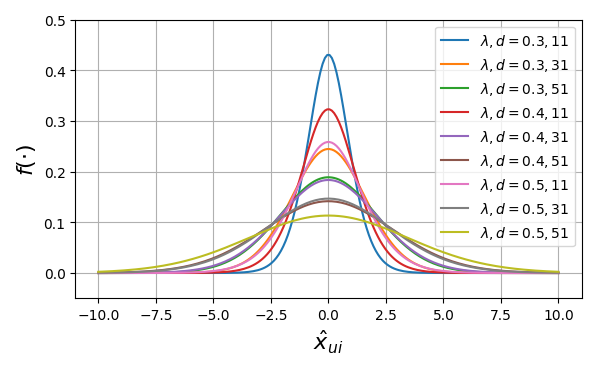
\includegraphics[width=.6\textwidth]{2-PriorPDF.png}}\\
	\subfloat{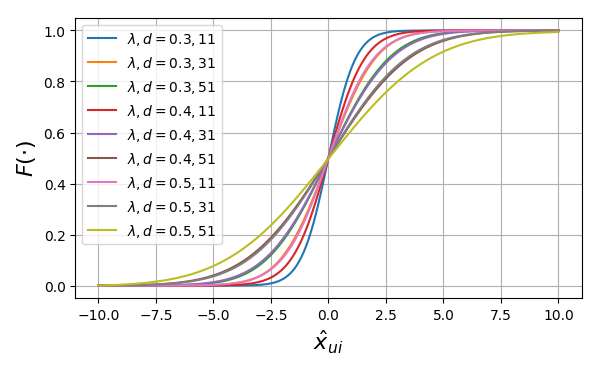
\includegraphics[width=.6\textwidth]{2-PriorCDF.png}}
	\caption{不同参数下先验分布的概率密度及累积分布函数示意图}
	\label{Fig:Prior}
\end{figure*}

\subsection{真正例相似度分数的分布}\label{Sec:Posterior}
本节的目标是获取真正例相似度观测值的分布。
%考虑$n$个独立同分布的随机变量$\{Z_i\}_{i=1}^n$,其对应的取值$\{z_i\}_{i=1}^n$按升序排列:$X_1 \le X_2 \le \cdots X_n$,其中$X_k$是取值$x_k$在第$k$个位置的随机变量,那么$x_k$的概率密度为
%\begin{equation}\label{Eq:PosteriorPDF}
%	\begin{aligned}
%		g({x_k};k,n)
%		=   \frac{{n!}}{{(k - 1)!(n - k)!}} {[\Phi({x_k})]^{k - 1}}\phi({x_k}){[1 - \Phi({x_k})]^{n - k}}.
%	\end{aligned}
%\end{equation}
对于一个交互,只存在两种可能:(1)它是真正例,即用户真的喜欢;(2)它是伪正例,即用户不喜欢。预测评分只存在两个总体,于是取$n=2$。此外,模型是针对负例评分小于正例评分优化,对于真正例的预测评分$\hat{x}_{ui}$,如果它是用户喜欢的正例,应该满足$\hat{x}_{uj}\leq \hat{x}_{ui}$。把这两个随机变量按升序排列,真正例的预测评分$\hat{x}_{ui}$在两个随机变量中排序第二,这正是次序统计量$X_{(2)}$的取值。根据第\ref{cha:intro1}章第\ref{order}部分关于次序统计量的预备知识,可以写出真正例的预测评分$\hat{x}_{ui}$的分布
\begin{eqnarray}\label{Eq:ConditionalDistribution}
	g(\hat{x}_{ui};k=2,n=2)
	& = & 2 F(\hat{x}_{ui})f(\hat{x}_{ui}),
\end{eqnarray}
其中 $f(\cdot)$由公式\ref{Eq:PDFInnerProduct}给出,$F(\cdot)$由公式\ref{Eq:CDFInnerProduct}给出。

图\ref{Fig:Posterior}绘制了不同参数下,可信交互(真正例)预测偏好值的分布示意图,可以看到它也满足概率分布的非负性和归一性条件。

\begin{figure*}[t]
	\centering
	\subfloat{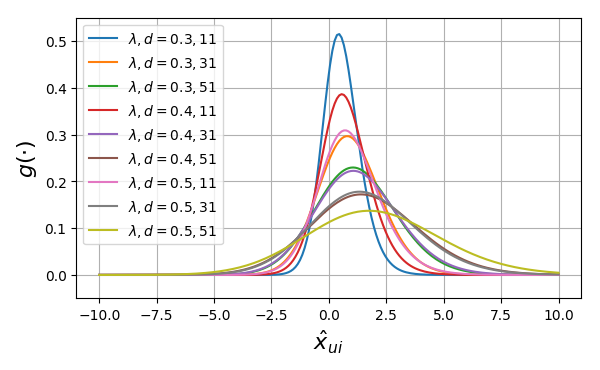
\includegraphics[width=.6\textwidth]{2-PosteriorPDF.png}}\\
	\subfloat{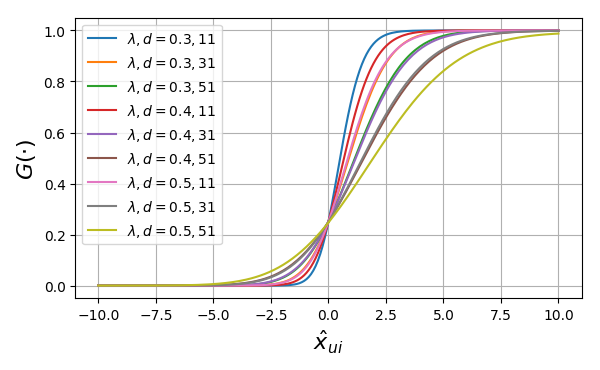
\includegraphics[width=.6\textwidth]{2-PosteriorCDF.png}}
	\caption{不同参数下后验分布的概率密度及累积分布函数示意图}
	\label{Fig:Posterior}
\end{figure*}

\subsection{学习算法}
在本节中,介绍自适应去噪的成对排序学习算法,并分析了其收敛性。由于这是一个含有隐变量的最大后验估计问题,因此使用EM算法\cite{Dempster:1977:RSS}进行端到端地估计隐变量并学习模型参数。具体而言,包括两个步骤:(i) 在期望步骤中估计$c_{ui}$,以及(ii) 在最大化步骤中学习用户和物品表示$\Theta$。

\subsubsection{期望步骤}
\newpage
在期望步骤中,固定的模型参数$\Theta$,即给定预测评分,目标是估计$c_{ui}$。首先写出$Q(\cdot)$函数\cite{Dempster:1977:RSS}为 
\begin{eqnarray}\label{Eq:QDef}
 Q(\Theta, \Theta^{(t)}) 
	& = & \mathbb{E}_{c_{ui} } \left[ \ln P(\Theta|\succ_u, c_{ui}) | \succ_u, \Theta^{(t)} \right] \nonumber \\
	& = & \mathbb{E}_{c_{ui}} \left[ \Sigma_{(u,i,j)\in \mathcal{D}} c_{ui} \left( \ln \sigma(\hat{x}_{ui} - \hat{x}_{uj}) - \lambda \| \Theta \|^2 \right) \right] \nonumber \\
	& = & \Sigma_{(u,i,j) \in \mathcal{D}} \mathbb{E}[c_{ui}] \left[ \ln \sigma(\hat{x}_{ui} - \hat{x}_{uj}) - \lambda \| \Theta \|^2 \right],
\end{eqnarray}
其中,$\mathbb{E}[c_{ui}]$是给定在第$t$次学习迭代中模型参数$\Theta^{(t)}$的条件下,$c_{ui}$的期望值。使用$\mathbb{E}[c_{ui}]$作为$c_{ui}$的估计。由于$c_{ui}$是一个二值伯努利变量,有以下关系式:

\begin{align}
 \hat{c}_{ui}=	\mathbb{E}[c_{ui}] &= P({c_{ui}} = 1|\Theta,{ \succ _u}) \nonumber \\
	&= P({c_{ui}} = 1|{\hat{x}_{ui}} ,\succ_u)  \label{Eq:EStimationCui} \\
	&= \frac{ P( {\hat{x}_{ui}},{ \succ_u}|{c_{ui}} = 1)}{ P({\hat{x}_{ui}} ,\succ_u)}{P({c_{ui}} = 1)} \label{Eq:Bayes}\\
	&\propto P( {\hat{x}_{ui}},{ \succ_u}|{c_{ui}} = 1)P({c_{ui}} = 1) \label{Eq:Bayesian} \\
	&= g({{\hat x}_{ui};n=2,k=2})P({c_{ui}} = 1) \label{Eq:ClassDensity}
\end{align}
$\succ_u$是BPR\cite{Steffen:2009:UAI}所定义的偏好结构,意为$\hat{x}_{uj}\leq \hat{x}_{ui}$。当固定模型参数$\Theta$时,预测评分$\hat{x}_{ui}$也被固定,于是有公式\eqref{Eq:EStimationCui}。式\eqref{Eq:Bayes}是基于贝叶斯公式得到,其中$P(c_{ui}=1)$是交互为可信的先验概率,分母$P(\hat{x}_{ui},\succ_u)$在贝叶斯分析中被省略为归一化常数。$P(\hat{x}_{ui},\succ_u|c_{ui}=1)$是可信交互的概率密度。给定所有的预测评分,对于一个可信的交互$(u,i)$,其预测评分$\hat{x}_{ui}$应该满足$\hat{x}_{uj} \leq \hat{x}_{ui}$,此时概率密度由公式\eqref{Eq:ConditionalDistribution}给出。在给定$P(c_{ui}=1)$的情况下,观测值$\hat{x}_{ui}$在分布$g({{\hat x}_{ui};n=2,k=2})$中对应的概率密度越高,它是可信交互的可能性越大。

设$n_i$表示物品$i$的选择比例,即与该物品进行交互的用户的百分比。令$\bar{n}$和$\sigma_n$分别表示交互比例的平均值和标准差。通过以下方式计算$P(c_{ui} =1)$:
\begin{eqnarray}
	P(c_{ui} =1) = \mathsf{sigmoid}(\frac{n_i - \bar{n} }{\sigma_n}).
\end{eqnarray}
其中$\mathsf{sigmoid}$函数的作用是将输入转换为$(0,1)$范围内的概率。该公式的直观解释是,一个物品的交互比例越高,越多用户交互,那么它是可信交互的先验概率越大。

\subsection{最大化步骤}
在最大化步骤中,固定隐变量$\hat{c}_{ui}$, 然后学习模型参数$\Theta$以最大化$Q(\cdot)$函数,即
\begin{equation}\label{Eq:MaxQFunction}
	\arg \mathop {\max }\limits_\Theta  \sum\nolimits_{(u,i,j) \in \mathcal{D}} {{{\hat c}_{ui}}[\ln \sigma ({{\hat x}_{ui}} - {{\hat x}_{uj}}) - {\lambda  }\|\Theta\|^2]}.
\end{equation}

\par
采用广泛使用的随机梯度下降(SGD)技术来学习模型参数。对于每个训练三元组$(u,i,j)$,其梯度为:
\begin{equation}\label{Eq:Gradient1}
	\frac{{\partial Q(\Theta, \Theta^{(t)} )}}{{\partial \Theta }} = \sum\nolimits_{(u,i,j) \in \mathcal{D}} \hat{c}_{ui} [ (1 - \sigma(\hat{x}_{ui}-\hat{x}_{uj}))\frac{\partial\hat{x}_{uij}}{\partial\Theta} - \lambda\Theta ],
\end{equation}
其中
\begin{equation}\label{Eq:Gradient2}
	\frac{{\partial {{\hat x}_{uij}}}}{{\partial \Theta }} = \frac{{\partial ({{\hat x}_{ui}} - {{\hat x}_{uj}})}}{{\partial \Theta }} = \left\{ {\begin{array}{*{20}{l}}
			{\mathbf{h}}_i - \mathbf{h}_j,\\
			{\mathbf{w}}_{u},\\
			{ - \mathbf{w}}_{u},
		\end{array}\begin{array}{*{20}{l}}
			{\mathrm{if} \;\; \theta  = {\mathbf{w}}_u}\\
			{\mathrm{if} \;\; \theta  = {\mathbf{h}}_i}\\
			{\mathrm{if} \;\; \theta  = {\mathbf{h}}_j}.
	\end{array}} \right.
\end{equation}
$\theta$表示$\mathbf{W}$或$\mathbf{H}$的特定行或者列。给定正则化参数$\alpha$,以及正则化常数$\lambda$,模型参数的更新规则为
\begin{equation}\label{Eq:Updating}
	\Theta  \leftarrow \Theta  + \alpha \hat{c}_{ui} [ (1 - \sigma(\hat{x}_{ui}-\hat{x}_{uj}))\frac{\partial\hat{x}_{uij}}{\partial\Theta} - \lambda\Theta ].
\end{equation}
\section{算法实现与时间复杂度分析}
\subsection{伪代码}
从公式\eqref{Eq:Updating}可以看出,新的参数$c_{ui}$充当了动态学习率的角色,实质上重新加权了具有较高偏好水平的交互,并为学习算法过滤了具有较低偏好水平的噪声交互。算法的实现使用了EM框架,在E步固定模型参数求解隐变量,在M步固定隐变量学习模型参数。算法~\ref{Alg2:1}给出了BPRAC学习算法的伪代码。
\begin{algorithm}[t]
	\counterwithin{algorithm}{chapter}
	\SetKwInput{KwIn}{输入}  %<---细节与重点
	\SetKwInput{KwOut}{输出}  %<---细节与重点
	\SetAlgoLined
	\small
	\caption{自适应去噪的成对学习排序算法伪码}\label{Alg2:1}
	\KwIn{交互集合$\mathcal{S}$, 训练三元组集合$\mathcal{D}$, 最大迭代轮数$T$, 抽样的训练三元组数量$K$。}
	\KwOut{预测的评分矩阵$\mathbf{X} \in \mathbb{R}^{M \times N}$。}
	初始化特征表示$\Theta =(\mathbf{W}, \mathbf{H})$,其中$\mathbf{w}_u \sim \mathcal{N}(0, \lambda \mathbf{I})$,$\mathbf{h}_i \sim \mathcal{N}(0, \lambda \mathbf{I})$ ;
	
	\For{$t = 1; t \le T; t$++}
	{
		\textit{\# Expectation步: 固定$\Theta$, 计算隐变量${{\hat c}_{ui}}$};
		
		\For{每一个交互$(u,i) \in \mathcal{S}$}
		{
			~~计算预测评分${{\hat x}_{ui}} = \left\langle   {{\mathbf{w}_u},{\mathbf{h}_i}} \right\rangle  $;\\
			通过公式~\eqref{Eq:PDFInnerProduct}计算先验分布$f({{\hat x}_{ui}})$;\\
			通过公式~\eqref{Eq:CDFInnerProduct}计算$F({{\hat x}_{ui}})$ ;\\
			通过公式~\eqref{Eq:ConditionalDistribution}计算后验分布$g({{\hat x}_{ui}};k=2,n=2)$;\\
			通过公式~\eqref{Eq:ClassDensity}计算${{\hat c}_{ui}}$;
		}
		\textit{\# Maximization步: 固定${{\hat c}_{ui}}$, 更新参数$\Theta$};
		
		\For{$k=1; k\le K; k$++}
		{
			~~抽样一个三元组$(u,i,j) \in \mathcal{D}$;\\
			计算预测评分${{\hat x}_{ui}}$,${{\hat x}_{uj}}$ ;\\
			通过公式~\eqref{Eq:Updating}执行梯度下降更新参数$\Theta$;
		}
	}
	\KwResult{$\mathbf{X}=\mathbf{W}\times {\mathbf{H}^\mathsf{T}} $。}
\end{algorithm}

\subsection{时间复杂度分析}
由于E步对隐变量的估计是标量计算,因此时间复杂度是$\mathcal{O}(|\mathcal{S}|)$,其中$|\mathcal{S}|$是训练集中交互总数。而M步主要是向量的梯度下降,因此M步的时间复杂度是$\mathcal{O}(|\mathcal{D}|d)$,其中,$|\mathcal{D}|$是三元组的数量,$d$是嵌入的维度。由于$|\mathcal{S}| \le\le (|\mathcal{D}|)$,即交互数远小于训练三元组的数量,因此自适应去噪的成对排序算法的时间复杂度主要源自于M步:固定隐变量,学习用户和物品的特征表示,即执行一次最外层循环的时间复杂度为$\mathcal{O}(|\mathcal{D}|d)$,这也是标准的BPR的时间复杂度。由于最外层要执行T次循环,总体的计算复杂度为$\mathcal{O}(T|\mathcal{D}|d)$,其中$T$是学习迭代的次数。

\section{收敛性分析}\label{Sec:Convergence}
在期望步骤中,使用$\mathbb{E}[c_{ui}] \propto \hat{c}_{ui}$的近似来计算$c_{ui}$的估计值。从公式\eqref{Eq:Updating}中可以直观地观察到,由于$\hat{c}_{ui} \ge 0$,$\hat{c}_{ui}$的近似仅改变参数更新过程中的步长,而不改变参数更新的方向,也就是说这个近似只改变了梯度下降过程中通往(局部)最小值的步长,但并不会改变梯度更新的方向,因此并不会改变算法的收敛性。BPRAC算法的收敛性的严格证明由如下引理给出。
\begin{lemma}\label{Lemma:ConvergenceAnalysis}
给定所有的成对比较 ${\succ _u}$,记后验概率序列为$P(\Theta^{(t)} |\succ_u)$,其中${\Theta ^{(t)}}(t=1,2,...)$为第$t$训练轮次学到的用户物品表示。那么,后验概率${P(\Theta ^{(t)}|\succ_u)}$收敛,且
	\begin{equation}\label{Eq:PosteriorSupremum}
		\mathop {\lim }\limits_{t \to \infty } P({\Theta ^{(t)}}|{ \succ _u}) = \sup \{ P({\Theta ^{(t)}}|{ \succ _u}) | t \in \mathbb{N}\}.
	\end{equation}
\end{lemma}

\begin{proof}
首先证明$\mathbb{E}[c_{ui}] \propto {{\hat c}_{ui}} $的这个近似不改变后验概率序列的非递减性质,也就是说要证明
\begin{equation}\label{eq20}
	P({\Theta ^{(t + 1)}}|{ \succ _u}) \ge P({\Theta ^{(t)}}|{ \succ _u}).
\end{equation}

\par
根据全概率公式,有
\begin{equation}\label{eq21}
	\begin{split}
		P(\Theta |{ \succ _u}) &= \frac{{P(\Theta ,c|{ \succ _u})}}{{P(c|\Theta ,{ \succ _u})}}\\
		& = \frac{{P(\Theta |c,{ \succ _u})P(c|{ \succ _u})}}{{P(c|\Theta ,{ \succ _u})}}.
	\end{split}
\end{equation}
因此
\begin{equation}\label{eq22}
	\begin{aligned}
		\log P(\Theta |{ \succ _u}) = \log P(\Theta |c,{ \succ _u}) - \log P(c|\Theta ,{ \succ _u})
		+ \log P(c|{ \succ _u}).
	\end{aligned}
\end{equation}
定义:
\begin{equation}\label{eq23}
	\begin{split}
		Q(\Theta ,{\Theta ^{(t)}}) &= {\mathbb{E}_{{c_{ui}}}}[\log P(\Theta |c,{ \succ _u})|{ \succ _u},{\Theta ^{(t)}}],\\
		H(\Theta ,{\Theta ^{(t)}}) &= {\mathbb{E}_{{c_{ui}}}}[\log P(c|\Theta ,{ \succ _u})|{ \succ _u},{\Theta ^{(t)}}],\\
		K(\Theta ,{\Theta ^{(t)}}) &= {\mathbb{E}_{{c_{ui}}}}[\log P(c|{ \succ _u})|{ \succ _u},{\Theta ^{(t)}}].
	\end{split}
\end{equation}
于是
\begin{equation}\label{eq24}
	\log P(\Theta |{ \succ _u}) \buildrel \Delta \over = Q(\Theta ,{\Theta ^{(t)}}) - H(\Theta ,{\Theta ^{(t)}}) + K(\Theta ,{\Theta ^{(t)}}).
\end{equation}
那么后验概率序列的差值为:
\begin{equation}\label{eq25}
	\begin{aligned}
		\log P({\Theta ^{(t + 1)}}|{ \succ _u}) - \log P({\Theta ^{(t)}}|{ \succ _u})
		= [Q({\Theta ^{(t + 1)}},{\Theta ^{(t)}}) - Q({\Theta ^{(t)}},{\Theta ^{(t)}})] \\
		- [H({\Theta ^{(t + 1)}},{\Theta ^{(t)}}) - H({\Theta ^{(t)}},{\Theta ^{(t)}})].
	\end{aligned}
\end{equation}

\par
在期望步骤中,采用了$\mathbb{E}[c_{ui}] \propto \hat{c}_{ui}$的近似方法。假设$\hat{c}_{ui} = \text{const} \cdot \mathbb{E}[c_{ui}]$,其中$\text{const} > 0$。根据最大化步骤,
\begin{equation}\label{eq26}
	\begin{split}
		{\Theta ^{(t+1)}} =& \arg \mathop {\max }\limits_\Theta  \sum\nolimits_{(u,i,j) \in {D_S}} {{{\hat c}_{ui}}[\ln \sigma ({{\hat x}_{ui}} - {{\hat x}_{uj}})}
		{- {\lambda _\Theta }||\Theta |{|^2}]}
		\\=& \arg \mathop {\max }\limits_\Theta  \sum\nolimits_{(u,i,j) \in {D_S}} {const \cdot E({c_{ui}})[\ln \sigma ({{\hat x}_{ui}} }
		{- {{\hat x}_{uj} )}- {\lambda _\Theta }||\Theta |{|^2}]}
		\\=& \arg \mathop {\max }\limits_\Theta  const \cdot Q(\Theta ,{\Theta ^{(t)}}).
	\end{split}
\end{equation}
\par
如上所示,使得$const \cdot Q(\Theta ,{\Theta ^{(t)}})$最大化的${\Theta ^{(t + 1)}}$也同时使得$Q(\Theta ,{\Theta ^{(t)}})$最大化,即$ Q({\Theta ^{(t + 1)}},{\Theta ^{(t)}}) - Q({\Theta ^{(t)}},{\Theta ^{(t)}}) > 0$。因此,公式\eqref{eq25}的第一项是非负的。接下来,按照标准的EM算法\cite{Dempster:1977:RSS}完成证明。公式\eqref{eq25}的第二项是:
\begin{equation}\label{eq27}
	\begin{aligned}
		&[H({\Theta ^{(t + 1)}},{\Theta ^{(t)}}) - H({\Theta ^{(t)}},{\Theta ^{(t)}})]\\
		=& {\mathbb{E}_{{c_{ui}}}}[\log P(c|{ \succ _u},{\Theta ^{(t + 1)}})|{ \succ _u},{\Theta ^{(t)}}] -{\mathbb{E}_{{c_{ui}}}}[\log P(c|{ \succ _u},{\Theta ^{(t)}})|{ \succ _u},{\Theta ^{(t)}}]\\
		=& {\mathbb{E}_{{c_{ui}}}}[\log \frac{{P(c|{ \succ _u},{\Theta ^{(t + 1)}})}}{{P(c|{ \succ _u},{\Theta ^{(t)}})}}|{ \succ _u},{\Theta ^{(t)}}]\\
		\le& \log {\mathbb{E}_{{c_{ui}}}}[\frac{{P(c|{ \succ _u},{\Theta ^{(t + 1)}})}}{{P(c|{ \succ _u},{\Theta ^{(t)}})}}|{ \succ _u},{\Theta ^{(t)}}]\\
		=& \log \int {\frac{{P(c|{ \succ _u},{\Theta ^{(t + 1)}})}}{{P(c|{ \succ _u},{\Theta ^{(t)}})}}P(c|{ \succ _u},{\Theta ^{(t)}})} dc\\
		=& 0.
	\end{aligned}
\end{equation}

\par
根据公式(\eqref{eq26})和(\eqref{eq27}),得出结论公式(\eqref{eq25})是非负的,也就是说,后验概率序列$P({\Theta ^{(t)}}|{ \succ _u})$是非递减的。

\par
其次,$P({\Theta ^{(t)}}|{ \succ _u})$是观察到的成对比较的后验概率,因此
\begin{equation}\label{eq28}
	\begin{split}
		P({\Theta ^{(t)}}|{ \succ _u})\le 1.
	\end{split}
\end{equation}
由于$P({\Theta ^{(t)}}|{ \succ _u})$是非递减的,并且1是其上界之一,根据单调有界收敛定理,对于$t \in \mathbb{N}$,后验概率序列存在极限,并且
%公式27
\begin{equation}\label{eq28}
	\begin{split}
		\mathop {\lim }\limits_{t \to \infty } P({\Theta ^{(t)}}|{ \succ _u}) = \sup \{ P({\Theta ^{(t)}}|{ \succ _u})| t \in \mathbb{N}\}.
	\end{split}
\end{equation}
证毕。
\end{proof}

\section{实验结果及分析}
\subsection{实验设置}
\subsubsection{数据集}
为了更好地评估所提出地算法能否更好地捕捉用户的兴趣偏好,测试集中的物品应该都是由用户喜欢的物品组成的“干净”测试集。在隐式反馈数据集中,无法构建“干净”的测试集,因为随机划分形成的测试集可能会包含噪声数据。而包含评分的数据集则可以实现这一目标,可以通过随机选择偏好值较高的物品构造“干净”的测试集。另一方面,在期望步骤中,学习到隐变量$c_{ui}$,是模型输出的用户对物品偏好值的大小。而包含真实偏好值的评分数据集可以用于评估隐变量$c_{ui}$估计的好坏。基于上述原因,本章的在三个广泛使用的评分数据集上进行实验,包括MovieLens-100k、MovieLens-1M和Yahoo!-R3 \cite{Xuejiao:2020:ASC}。它们包含用户对物品的评分,最满意为五分,最不满意为一分。评分信息仅用于构建由用户喜欢的物品组成的“干净”测试集,并用于评估隐变量$c_{ui}$估计的好坏,并不会用来训练。

具体而言,训练集和测试集的划分方法如下:对于MovieLens-100K和MovieLens-1M数据集,对于每个五分评分的物品,随机选择50%的物品作为测试数据。而Yahoo!-R3数据集中,五分评分的物品很少。为了避免测试集中物品过少,随机选择50%的评分大于三分的物品\cite{Wang:2021:WSDM}作为测试数据,因为这样的歌曲也能反映出一定程度的用户偏好。剩余的数据构成了训练集。因此,训练集中包含大量评分为一分的用户不喜欢的物品,即噪声。在模型训练时,将所有评分抹去,转换为隐式反馈 \cite{Steffen:2009:UAI,Zhao:2019:FGCS,Yu:2018:CIKM},不使用任何评分数据。表~\ref{Table:Dataset}总结了数据集的统计信息。

\begin{table}[t]
	\centering
	\caption{数据集统计信息}\label{Table:Dataset}
	\begin{tabular}{lrrrrr}
		\toprule[0.5pt]
		数据集           & 用户数   & 物品数   & 训练集交互数  &测试集交互数& 密度  \\ \cline{1-6}
		ML-100k   &   943    &  1,682   &    89,372	   & 10,628&  6.30\%	\\
		ML-1M    &   6,040  &  3,952   &   887,007      & 113,202 &4.19\%  \\
		Yahoo!-R3       &   5,400  &  1,000   &   129,180      & 12,520&2.62\%  \\
		\bottomrule[0.5pt]
	\end{tabular}%
\end{table}

\subsubsection{对比方法}
本章提出的自适应去噪的成对排序推荐算法(Bayesian Personalized Ranking with Autonomous Credence, BPRAC)旨在从含噪成对比较中学习排序,因此同类对比方法主要为含有去噪机制的成对学习算法。
\begin{itemize}
\item BPR~\cite{Steffen:2009:UAI}(UAI, 2008):BPR在本文中已经被很好地介绍过。该方法提供了在没有去噪机制情况下,伪正例问题对准确学习用户偏好的负面影响,是一个重要的消融实验结果。
\item GBPR~\cite{Weike:2013:IJCAI}(IJCAI, 2013):GBPR为用户$u$通过群体偏好的概念$\mathcal{G}(i)$引入了更可靠的自监督信号,有助于对抗伪正例问题。其中$\mathcal{G}(i)$是与物品$i$有交互的其他用户的群体偏好估计值。该方法将优化目标修改为“对已交互物品的群体偏好大于对负例的偏好”。由于群体偏好是多个用户对物品$i$偏好的平均值,其中包含的噪声影响会被稀释。这一优化目标相对于单个用户的偏好结构更加稳定和鲁棒,有助于对抗正例中的噪声。

\item MPR~\cite{Yu:2018:CIKM}(CIKM, 2018):MPR构建了更细粒度的偏好比较,将优化目标细分为正例、未交互物品和不喜欢的物品三种类型,构建了如下优化目标:$r_{ui} - r_{uj_2} \geq r_{uj_1} - r_{uj_2} \geq r_{ui_1} - r_{ui_2}$,$i,i_1,i_2 \in \mathcal{I}_u^+$,$j_1, j_2 \in \mathcal{I}_u^-$,其中$j_1$是未交互但可能喜欢的物品,$j_2$是用户不喜欢的物品,从最不受欢迎的物品(交互频率最低的物品)中选择。这个优化目标由两部分构成,即$r_{ui} - r_{uj_2} \geq r_{uj_1} - r_{uj_2} $和$ r_{uj_1} - r_{uj_2} \geq r_{ui_1} - r_{ui_2}$,即使伪正例问题会造成第一个优化目标的错误,但是第二个优化目标仍然是正确的,这种更细粒度的自监督信号在一定程度上缓解伪正例问题导致的模型误判用户的兴趣边界。

\item DenoiseRec~\cite{Wang:2021:WSDM}(WSDM, 2021):DenoiseRec是一个专门针对伪正例问题设计的推荐算法,该方法率先在推荐系统中引入小损失技巧,其核心思想是损失值较大的样本可能是噪声。具体而言,该方法预定义一个阈值$\tau$,对于那些大于$\tau$的损失值的样本,DenoiseRec认为很有可能是噪声交互,并使用动态阈值函数将损失值截断为0,或者使用较小的权重进行重新加权。
\end{itemize}

\subsubsection{参数设置}
模型的超参数$d$和$\lambda$在对比算法中已经进行了详细讨论\cite{Steffen:2009:UAI,Weike:2013:IJCAI,Yu:2018:CIKM}。遵循它们的讨论,在三个数据集中将$d$设置为27,并在Movielens-1K和Movielens-1M数据集中将$\lambda$设置为0.6,在Yahoo!-R3数据集中将$\lambda$设置为0.2。将迭代次数$T=10$,学习率$\alpha=0.05$,采样的三元组数量$K=1000 \times$用户数量,对于所有三个数据集保持一致。对比算法中的其他超参数是根据其AUC指标的最佳性能进行选择的。

按照BPR~\cite{Steffen:2009:UAI}的做法,采用广泛使用的AUC作为衡量模型的收敛性以及推荐列表的质量。此外,还采用常用的用于Top-K个性化推荐的评估指标,包括Precision、Recall、F1、NDCG(归一化折现累积增益)和MAP(平均准确率)。由于评估指标的广泛使用,受限于篇幅,详细定义参考\cite{ml:2018}。

\subsection{实验结果及分析}
\subsubsection{$\hat{c}_{ui}$的估计质量}
估计$\hat{c}_{ui}$的任务可以直观理解为预测隐式反馈数据集中每个交互对应的偏好值大小的过程,也可以看作是对不完全的隐式反馈数据集的(Incomplete Data)数据恢复过程。$\hat{c}_{ui}$的预测值越高,交互被认为越可信,偏好值也就越高。在训练数据集中,评分则为真实标签,就可以根据评分来判定$\hat{c}_{ui}$估计质量的好坏。

特别地,把训练集中评分为1的交互设置为噪声交互,通过对比预测值和真实标签值,那么就可以绘制ROC曲线,以及计算隐变量的AUC值,从而对$\hat{c}_{ui}$的估计质量进行进行评估。据我们所知,这是首个在不完全数据的隐式反馈数据集上进行数据恢复的任务,因此只汇报BPRAC算法的隐变量的估计质量。
\begin{figure}[!]
	\centering
	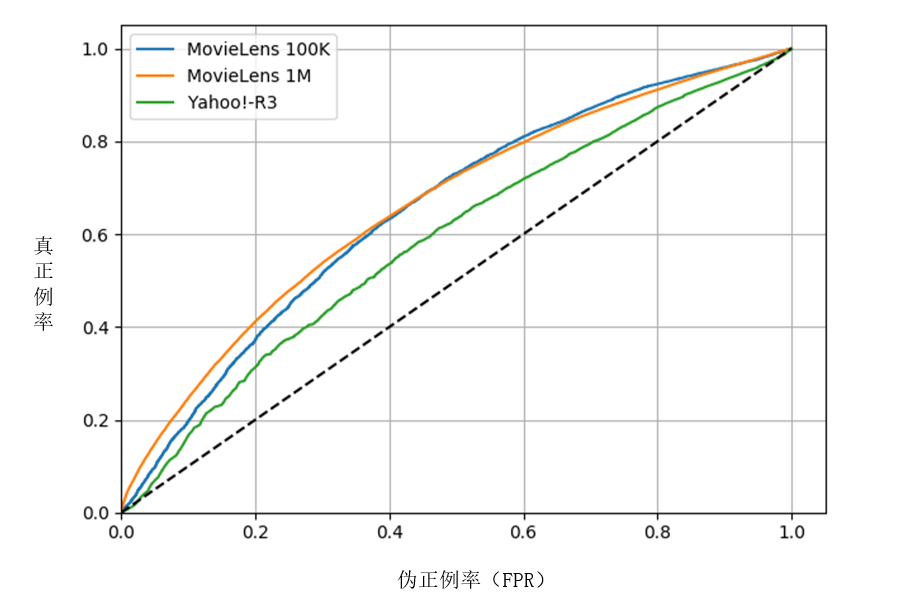
\includegraphics[width=0.7\textwidth]{2-roc.png}
	\caption{隐变量估计的ROC曲线}
	\label{Fig:ROC}
\end{figure}
\begin{table}[!]
	\centering
	\caption{隐变量的估计质量}\label{Table:ActionRecognition}
	\begin{tabular}{cccc}
		\toprule[1.2pt]
		数据集            & MovieLens-100k &	MovieLens-1M & Yahoo!-R3 \\ \hline
		AUC               & 0.6524       &  0.6618        & 0.5885 \\
		\bottomrule[1.2pt]
	\end{tabular}
\end{table}
图~\ref{Fig:ROC}绘制了通过不同估计阈值的所有交互的$\hat{c}_{ui}$的ROC(接收者操作特性)曲线,并且表~\ref{Table:ActionRecognition}计算了三个数据集对应的AUC。首先,$\hat{c}_{ui}$的AUC性能并不是很令人满意,但它们仍然比简单猜测抛硬币要好,显著大于50\%。这意味着,BPRAC算法总体上能够为偏好较高的交互输出一个较大的$\hat{c}_{ui}$估计值,为偏好较低的交互输出一个较小的$\hat{c}_{ui}$估计值。

为真实评分较高的物品输出一个较大的$\hat{c}_{ui}$预测值,使得模型从该物品学习更多信息;为真实评分较小的物品输出一个较小的$\hat{c}_{ui}$预测值,避免模型从噪声中学习到错误的信息,从而误判用户的兴趣偏好。在仅具有二元交互的有限信息下,$\hat{c}_{ui}$估计的有效性主要来自于次序统计量,它导致了后验分布的收窄,从而减小了随机变量的不确定性,如公式~\eqref{Eq:Bayesian}所描述。
\par 
\subsubsection{个性化推荐性能} 

表~\ref{Table:Recommendation}比较了五种成对学习排序模型的个性化性能。首先,BPRAC模型在所有评估指标中表现最好,这得益于隐变量的引入。在E步,由于BPRAC算法总体上能够为偏好较高的交互输出一个较大的$\hat{c}_{ui}$估计值,为偏好较低的交互输出一个较小的$\hat{c}_{ui}$估计值,使得模型从可靠的交互学到更多信息,且避免从噪声中学到错误信息,从而更准确地学习用户的偏好,产生更准确的预测。其次,此外,BPR表现不佳,该方法没有在隐式反馈数据中的去噪机制,每个交互都被认为是体现用户偏好的交互,这显然是不符合实际情况的。该消融实验结果表明噪声交互的存在对成对学习模型产生了不利影响,验证了在隐式反馈数据集中去噪的必要性。再次,DenoiseRec通过引入小损失的技巧来降低噪声,取得了次优的结果,这说明小损失技巧对于成对学习算法也是适用的;然而,与BPRAC相比,DenoiseRec收敛到一个较小的AUC值。在去噪机制方面,二者的唯一差异在于权重的计算机制不同:在BPRAC方法中,权重,即隐变量$\hat{c}_{ui}$是自适应学到的;而在DenoiseRec方法中,权重是手动设计的。手动设计权重依赖于密集的调参;另一方面,手动设计的权重通过下加权损失值较大的样本,削弱了困难负样本对学习算法的贡献。因为较大的损失值,可能是由于困难负样本所导致的。因此,自适应的参数学习比经验地手动设置权值更有效。

\begin{table*}[!]
	\centering
	\caption{Top-k 推荐性能比较}\label{Table:Recommendation}
	\resizebox{1\textwidth}{!}{
		\begin{tabular}{llccccccccccc}
			\toprule[1.2pt]
			\multirow{2}*{\textbf{数据集}} & \multirow{2}*{\textbf{方法}}  & \multicolumn{5}{c}{Top-5评估} &~& \multicolumn{5}{c}{Top-10评估}\\ \cline{3-7} \cline{9-13}
			~&~ & Precision & Recall & F1 & NDCG & MAP&~ & Precision & Recall & F1 & NDCG & MAP \\ \cline{1-7} \cline{9-13}
			\multirow{4}*{MovieLens-100K} & BPR & 0.2888 & 0.1897 & 0.1818 & 0.3401 &0.4893 &~  & 0.2379 & 0.2923 & 0.2075 & 0.3422 & 0.4663  \\
			~ & GBPR & 0.2976 & 0.1944 & 0.1872 & 0.3504 &0.4967&~ & 0.2458 & 0.3031 & 0.2147 & 0.3538 & 0.4780 \\
			~ & MPR & 0.1224 & 0.0741 & 0.0754 &0.1333& 0.2278&~ & 0.1053 & 0.1331 & 0.0935 & 0.1412 & 0.2295  \\
			~ & DenoiseRec & \underline{0.3042} & \underline{0.1990} & \underline{0.1883} &\underline{0.3528}&\underline{0.5122}&~ & \underline{0.2541} & \underline{0.3027} & \underline{0.2192} & \underline{0.3553} & \underline{0.4955}  \\
			~& \textbf{BPRAC} & \textbf{0.3265} & \textbf{0.2158} &\textbf{0.2055}  & \textbf{0.3879} &\textbf{0.5393} &~ & \textbf{0.2665} & \textbf{0.3216} &\textbf{0.2305} & \textbf{0.3859} &\textbf{0.5127}  \\ \cline{1-7} \cline{9-13}
			
			\multirow{4}*{MovieLens-1M} & BPR & 0.2940 & 0.1086 & 0.1323 & 0.3148 &0.4645&~ & 0.2570 & 0.1825 & 0.1741 & 0.3042 & 0.4517  \\
			~& GBPR & 0.3119 & 0.1265 & 0.1497 & 0.3376 &0.5004 &~ & 0.2655 & 0.2027 & 0.1874 & 0.3235 & 0.4797 \\
			~& MPR & 0.1125 & 0.0410 & 0.0494 & 0.1212 &0.2226&~ & 0.1036 & 0.0713 & 0.0681 & 0.1207 & 0.2278 \\
			~ & DenoiseRec & \underline{0.3205} & \underline{0.1174} & \underline{0.1434} &\underline{0.3432}&\underline{0.4996}&~ &\underline{0.2737}&\underline{0.1901} & \underline{0.1831} & \underline{0.3257} & \underline{0.4783}  \\
			~& \textbf{BPRAC} & \textbf{0.3472} & \textbf{0.1282} & \textbf{0.1572} & \textbf{0.3721} &\textbf{0.5297} &~ & \textbf{0.2992} & \textbf{0.2110} & \textbf{0.2026} & \textbf{0.3559} & \textbf{0.5044}  \\\cline{1-7} \cline{9-13}
			
			\multirow{4}*{Yahoo!-R3} & BPR & 0.0861 & 0.1007 & 0.0840 & 0.1099 & 0.1890 &~ & 0.0685 & 0.1566 & 0.0875 & 0.1284 & 0.1962  \\
			~ & GBPR & 0.1044 &0.1250 & 0.1037 & 0.1343 &0.2292&~ & 0.0817 &0.1943 & 0.1063 & 0.1576 & 0.2351  \\
			~ & MPR & 0.0694 & 0.0642 & 0.0511 & 0.0744 &0.1353&~ &0.0551 & 0.1095 & 0.0527 & 0.0875 & 0.1503  \\
			~ & DenoiseRec & \underline{0.1058} & \underline{0.1257} & \underline{0.1042}&\underline{0.1349}&\underline{0.2247}&~ & \underline{0.0841} & \underline{0.1993} & \underline{0.1086} & \underline{0.1596} & \underline{0.2326}  \\
			
			~& \textbf{BPRAC} & \textbf{0.1117} & \textbf{0.1308} & \textbf{0.1096} & \textbf{0.1448} &\textbf{0.2465}&~  & \textbf{0.0857} &\textbf{0.2034} & \textbf{0.1109} & \textbf{0.1675} & \textbf{0.2510} \\
			\bottomrule[1.2pt]
		\end{tabular}
	}
\end{table*}


\subsubsection{对噪声数据的敏感性}
图~\ref{Fig:impactd}展示了BPRAC算法对不同噪声率地敏感性。通过训练集中随机生成噪声数据,可以模拟训练集中含有更高噪声交互的情况。以噪声率控制数据集中噪声数据的比例,生成包含噪声的训练集时,不同的学习算法使用相同的含有噪声的训练集训练。对比方法选择BPR和DenoiseRec。如图~\ref{Fig:impactd}所示,噪声率的增加导致三种学习算法的个性化推荐性能都下降,表明噪声交互的存在对学习模型产生不利影响,且噪声率越高,对准确学习用户偏好的不利影响越大;另一方面,由于BPRAC和DenoiseRec包含去噪机制,它们相对于BPR更具鲁棒性。此外,DenoiseRec的性能下降略多于BPRAC,这意味着通过自适应地学习置信度,比经验地手动设定权重更加有效。
\begin{figure*}[!]
	\centering
	\subfloat{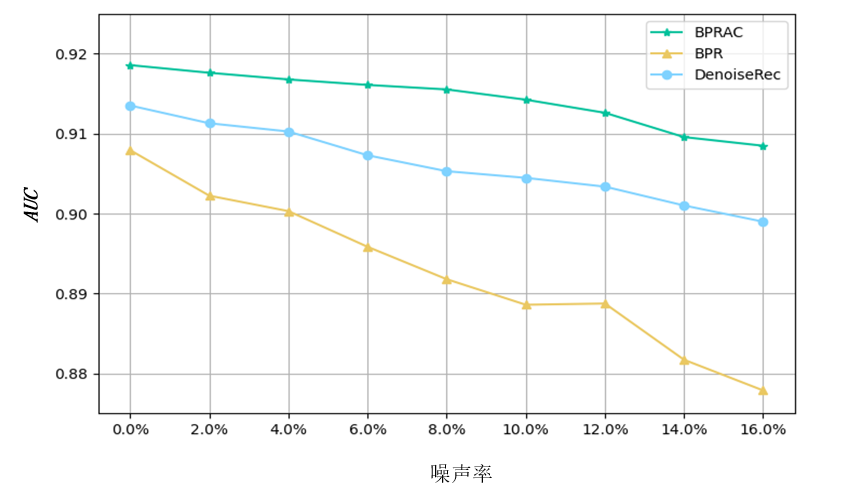
\includegraphics[width=.7\textwidth]{2-noisyratio.png}}
	\caption{不同噪声率对学习算法性能的影响}
	\label{Fig:impactd}
\end{figure*}
\par
\subsubsection{算法收敛性分析}
 图~\ref{Fig:Covergence}比较了五种算法的收敛性,度量指标为排序列表的AUC,这是因为成对损失函数可以类比于AUC指标\cite{Steffen:2009:UAI}。AUC指标的收敛意味着算法的收敛。首先观察到,所有算法的AUC在足够的训练迭代后首先增加,然后收敛。这个试验结果也印证了引理~\ref{Lemma:ConvergenceAnalysis}的分析,如公式~\eqref{Eq:PosteriorSupremum}所示。此外注意到,与对比算法相比,本章提出的的BPRAC收敛到一个更高的AUC指标,代价是更慢的收敛速率从而需要更多的训练轮次,通常需要比BPR多进行2-3倍更新,这是由于引入了新的隐藏变量$c_{ui}$。这个代价是值得的,因为BPRAC提供了一种从噪声数据中学习排序的解决方案。最后,专门针对噪声的DenoiseRec方法,由于引入了小损失技巧,把损失值较大的样本进行下加权,从而也降低了困难负样本对学习算法的贡献,因此也具有较慢的收敛速率,通常需要更多次的迭代。
\begin{figure}[!]
	\centering
	\subfloat{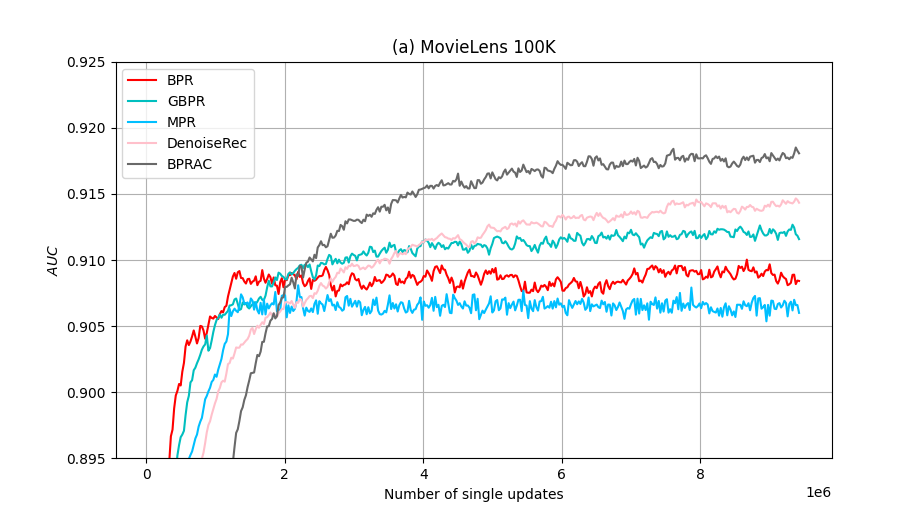
\includegraphics[width=.8\textwidth]{2-c100k.png}}\\
	\subfloat{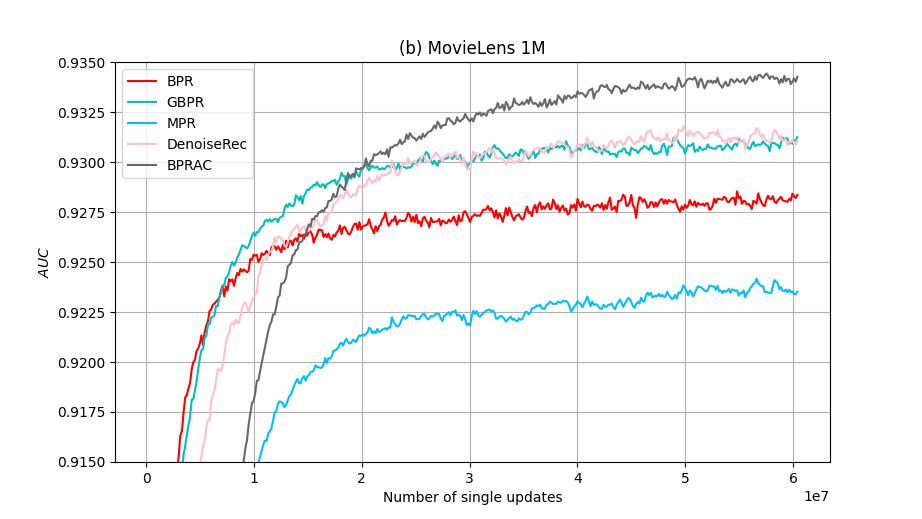
\includegraphics[width=.8\textwidth]{2-c1m.png}}\\
	\subfloat{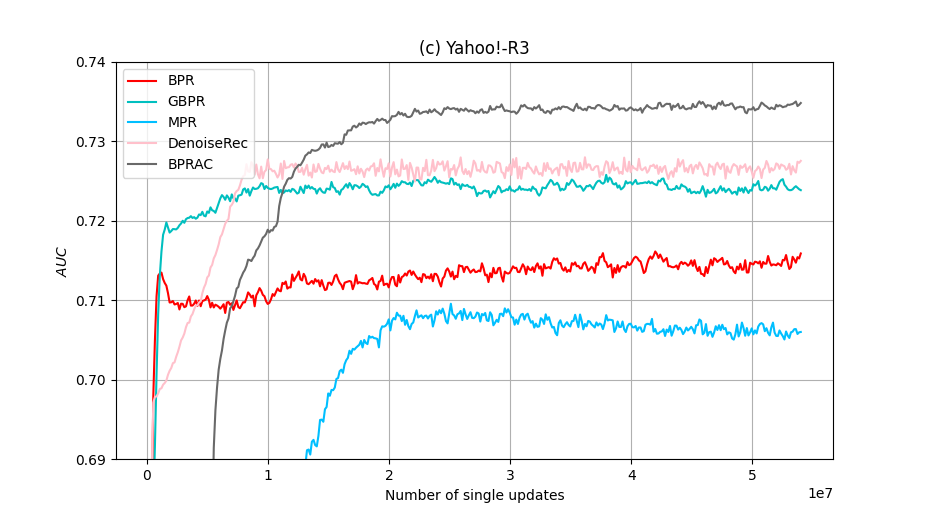
\includegraphics[width=.8\textwidth]{2-cyahoo.png}}
	\caption{不同学习算法的收敛速度比较}
	\label{Fig:Covergence}
\end{figure}

\section{本章小结}
本章聚焦于推荐系统的伪正例问题,研究了从含噪成对比较中学习排序的问题。由于隐式反馈是不完全数据,其中的伪正例构建的噪声成对比较,会对学习算法产生不利的影响。对于每个交互数据,本章引入了一个隐变量指示其可信度,并把从不完全数据中学习排序的问题形式化为一个含有隐变量的最大后验估计问题。针对这一问题,本章提出了自适应去噪的成对排序算法(BPRAC),端到端地估计隐变量并学习用户和物品表示。BPRAC算法在EM框架下求解:在E步固定模型参数估计隐变量,在M步固定隐变量学习模型参数。对真实的推荐数据集进行的实验BPRAC算法相对于其他对比方法的优越性。但是,相对于异常交互模式产生的伪正例问题,负例未标是隐式反馈数据面临的一个更突出问题,也是机器学习更具普遍性的问题。本章的研究将为后续章节中探索更复杂模型和更一般的伪负例场景的解决方案提供启示。